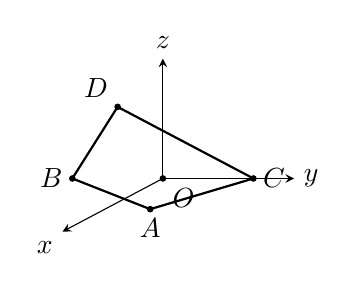
\begin{tikzpicture}[
  x={(-0.85cm,-0.45cm)}, y={(1.15cm,0cm)}, z={(0cm,1.05cm)},
  >=stealth,scale=1.0,line cap=round,line join=round]
  \coordinate (O) at (0,0,0);
  \coordinate (B) at (0,-1,0);
  \coordinate (C) at (0,1,0);
  \coordinate (A) at ({sqrt(3)/2},0.5,0);
  \coordinate (D) at (0,-0.5,{sqrt(3)/2});
  \draw[->] (O)--(1.5,0,0) node[below left] {$x$};
  \draw[->] (O)--(0,1.45,0) node[right] {$y$};
  \draw[->] (O)--(0,0,1.45) node[above] {$z$};
  \draw[thick] (B)--(D)--(C)--(A)--cycle;
  \fill (O) circle (1.2pt) node[below right] {$O$};
  \fill (A) circle (1.2pt) node[below] {$A$};
  \fill (B) circle (1.2pt) node[left] {$B$};
  \fill (C) circle (1.2pt) node[right] {$C$};
  \fill (D) circle (1.2pt) node[above left] {$D$};
\end{tikzpicture}
